\documentclass[11pt,a4paper]{article}

\usepackage[utf8]{inputenc}
\usepackage[margin=1in]{geometry}
\usepackage{amsmath,amssymb,amsfonts,amsthm}
\usepackage{booktabs}
\usepackage{graphicx}
\usepackage{hyperref}
\usepackage{url}
\def\UrlBreaks{\do\/\do-}
\usepackage{microtype}
\usepackage{xcolor}
\usepackage{caption}
\usepackage{subcaption}
\usepackage{natbib}
\usepackage{algorithm}
\usepackage{algorithmic}
\usepackage{multirow}

\hypersetup{
    colorlinks=true,
    linkcolor=blue!70!black,
    citecolor=green!50!black,
    urlcolor=blue!80!black
}

\graphicspath{{figures/}}

\newtheorem{theorem}{Theorem}
\newtheorem{lemma}[theorem]{Lemma}
\newtheorem{corollary}[theorem]{Corollary}

\title{\textbf{Denoised Gradient Estimation: \\ Training Deep Neural Networks Without Backpropagation via Coordinate Block Perturbations and Dual Sign-EMA Temporal Filtering}}

\author{
  \textbf{Mario Raúl Carbonell Martínez}\thanks{Corresponding author: \texttt{marioraulcarbonell@gmail.com}.\\Code and repository: \url{https://github.com/mcarbonell/dge-optimizer}.} \\
  Independent Researcher \\
  \texttt{marioraulcarbonell@gmail.com}
}

\date{October 2026}

\begin{document}

\maketitle

\begin{abstract}
Gradient-based optimization requires analytical derivatives, limiting its applicability to non-differentiable architectures, physical neuromorphic hardware, and black-box environments. We introduce \textbf{Denoised Gradient Estimation} (DGE), a zeroth-order algorithm that trains deep neural networks using only forward-pass evaluations. DGE combines three complementary mechanisms: (1)~\emph{coordinate block-wise perturbations} that reduce gradient variance by a factor of $K$, where $K$ is the number of active blocks; (2)~\emph{temporal exponential moving average} (EMA) filtering that improves signal-to-noise ratio as $\mathcal{O}(\sqrt{T})$; and (3)~a novel \emph{Dual Sign-EMA} (DS-EMA) consistency mask inspired by MACD crossover detection, achieving a 90\% memory reduction over sliding-window buffers. On full MNIST (60K samples, 109K parameters), DGE achieves \textbf{94.36\%~$\pm$~0.23\%} best test accuracy without backpropagation---reaching 96.3\% of Adam's peak performance. In non-differentiable settings where backpropagation fails entirely, DGE operates natively without straight-through estimators (STE), achieving \textbf{74.24\%} on INT8 and \textbf{68.82\%} on INT4 full quantization where backprop collapses to near random guessing ($\sim$9.8\%), and reaching \textbf{70.43\%} on discontinuous sign activations. We provide formal theoretical bounds establishing the estimator's unbiasedness, a $K$-fold variance reduction law, and temporal SNR convergence guarantees.
\end{abstract}

\vspace{0.5em}
\noindent\textbf{Keywords:} Zeroth-Order Optimization, Gradient-Free Training, Coordinate Block Perturbation, Temporal Consistency Filtering, Dual Sign-EMA, Non-Differentiable Neural Networks, Quantization-Aware Training.

\newpage

% -----------------------------------------------------------------------------
\section{Introduction}
\label{sec:intro}
% -----------------------------------------------------------------------------

Backpropagation is the foundational workhorse of modern deep learning~\citep{rumelhart1986learning,lecun2015deep}. However, its strict reliance on analytical derivatives limits applicability in several critical regimes: (i)~black-box systems where the objective function is an opaque oracle or physics simulator, (ii)~non-differentiable edge hardware such as neuromorphic or analog processors~\citep{schuman2022opportunities,davies2018loihi}, (iii)~discrete architectures including binary~\citep{yin2020binary} and ternary networks, and (iv)~memory-constrained settings where caching intermediate activation tensors for backward autodiff graphs is physically infeasible.

Zeroth-order (gradient-free) optimization methods estimate directional derivatives using only forward loss queries, offering a universal alternative. However, classical zeroth-order approaches confront a catastrophic dimensionality barrier. Simultaneous Perturbation Stochastic Approximation (SPSA)~\citep{spall1992multivariate} perturbs all $D$ parameters simultaneously, producing a gradient estimator whose variance scales linearly with dimensionality. In modern deep networks with $D > 10^5$ parameters, this cross-perturbation noise overwhelms the gradient signal, causing the optimizer to diverge or collapse~\citep{ghadimi2013optimal}.

Recent interest has revived zeroth-order methods for fine-tuning Large Language Models. MeZO~\citep{malladi2023mezo} achieves memory-efficient adaptation by regenerating perturbation vectors from a seed. Crucially, however, MeZO operates in the localized regime where heavily pre-trained models already reside near a basin of attraction---a setting fundamentally distinct from optimizing neural networks from scratch across high-dimensional non-convex landscapes.

\paragraph{Our approach.} We introduce \textbf{Denoised Gradient Estimation} (DGE), which resolves the high-dimensional variance catastrophe through three coupled principles:
\begin{enumerate}
    \item \textbf{Coordinate Block Perturbations:} Partition the $D$-dimensional parameter space into $K \ll D$ coordinate blocks per step, bounding cross-contamination noise by the block fraction $B/D = 1/K$ and reducing variance by a factor of $K$.
    \item \textbf{Temporal Denoising:} Inject sparse gradient estimates into an Adam-style EMA filter, exploiting the fact that coherent gradient signals accumulate constructively while independent cross-block noise sums destructively, yielding SNR improvement as $\mathcal{O}(\sqrt{T})$.
    \item \textbf{Dual Sign-EMA (DS-EMA):} A MACD-inspired directional consistency gate that tracks fast ($\alpha_f = 0.3$) and slow ($\alpha_s = 0.05$) sign trends, achieving a 90\% memory reduction over sliding-window buffers while suppressing non-stationary noise.
\end{enumerate}

\paragraph{Summary of Contributions.}
\begin{itemize}
    \item \textbf{Mathematical Foundations:} We prove that the coordinate block estimator is unbiased under first-order expansion and establish a $K$-fold variance reduction bound $\text{Var}(g_{t,i}) \leq \frac{1}{K} \|\nabla f\|^2$.
    \item \textbf{Dual Sign-EMA Filter:} We introduce DS-EMA, a constant-memory temporal consistency filter that identifies persistent descent directions and suppresses noise oscillations.
    \item \textbf{Empirical Validation on Vision:} On full MNIST (109K parameters), DGE achieves \textbf{94.36\%~$\pm$~0.23\%} best test accuracy without backpropagation, reaching 96.3\% of Adam's baseline.
    \item \textbf{Non-Differentiable Regimes:} In fully quantized networks (INT8 and INT4) and discontinuous sign activations without straight-through estimators, DGE achieves 68.8\%--74.2\% accuracy where Adam collapses to random guessing ($\sim$9.8\%).
    \item \textbf{Optimal Scaling Law:} We demonstrate theoretically and empirically that selecting block count $K = \mathcal{O}(\sqrt{D})$ provides the optimal bias-variance Pareto frontier for neural network training.
\end{itemize}

% -----------------------------------------------------------------------------
\section{Related Work}
\label{sec:related}
% -----------------------------------------------------------------------------

\paragraph{Finite Differences and Coordinate Descent.}
Classical finite difference methods compute exact numerical gradients via central differences: $g_i = (f(x + \delta e_i) - f(x - \delta e_i)) / (2\delta)$. However, evaluating all $D$ coordinates requires $2D$ forward passes per step, rendering it computationally intractable for deep neural networks with millions of parameters~\citep{nocedal2006numerical,bertsekas2019nonlinear}.

\paragraph{Simultaneous Perturbation Stochastic Approximation (SPSA).}
SPSA~\citep{spall1992multivariate} reduces function evaluations to two queries per step by perturbing all parameters simultaneously using a shared Rademacher vector. While the estimator is expectation-unbiased, its variance scales as $\mathcal{O}(D)$, leading to severe signal degradation and divergence in deep neural network parameter manifolds~\citep{ghadimi2013optimal}.

\paragraph{Evolution Strategies and Natural Evolution.}
OpenAI's Evolution Strategies (ES)~\citep{salimans2013evolution} and Natural Evolution Strategies (NES)~\citep{wierstra2014natural} conduct population-based search with Gaussian perturbations. While effective for reinforcement learning and policy search, they require $\mathcal{O}(\lambda)$ evaluations per generation for population size $\lambda$, and their throughput is constrained by high sample complexity on large datasets.

\paragraph{Forward Gradients and Memory-Efficient Zero-Order LLMs.}
Forward-mode automatic differentiation computes directional derivatives along random vectors~\citep{baydin2022survey}. MeZO~\citep{malladi2023mezo} adapted this for fine-tuning pre-trained language models with $\mathcal{O}(1)$ memory. However, because MeZO perturbs all dimensions simultaneously without coordinate partitioning, its gradient variance remains $\mathcal{O}(D)$, leading to collapse when attempting to train randomly initialized deep architectures from scratch.

\paragraph{Training Non-Differentiable Architectures.}
Optimizing neural networks with discrete weights or discontinuous step activations conventionally relies on straight-through estimators (STE)~\citep{bengio2013estimating} or surrogate gradient approximations. DGE completely sidesteps these heuristics, treating the objective as a genuine black-box landscape.

% -----------------------------------------------------------------------------
\section{Methodology: Denoised Gradient Estimation}
\label{sec:method}
% -----------------------------------------------------------------------------

We consider the unconstrained optimization problem $\min_{x \in \mathbb{R}^D} f(x)$, where $f$ can be evaluated via forward inference passes, but analytical gradients $\nabla f$ are inaccessible or nonexistent.

\subsection{Coordinate Block Perturbations}
\label{sec:blocks}

At step $t$, DGE generates a uniform random coordinate partition $\pi_t$ of $\{1, \dots, D\}$ into $K$ disjoint blocks $B_1, \dots, B_K$ of size $B = D/K$. For each block $B_k$, we sample a Rademacher vector $s_t^{(k)} \in \{-1, +1\}^{|B_k|}$ and compute the symmetric two-point query:
\begin{equation}
    g_{t,i} = \frac{f(x_t + \delta \cdot s_t^{(k)} \odot m_k) - f(x_t - \delta \cdot s_t^{(k)} \odot m_k)}{2\delta} \cdot s_{t,i}^{(k)}, \quad i \in B_k,
    \label{eq:block_estimator}
\end{equation}
where $m_k \in \{0, 1\}^D$ is the binary indicator vector for block $B_k$, and $\delta > 0$ is the perturbation magnitude. Evaluating all $K$ blocks requires $2K$ function evaluations per step. Because all $2K$ perturbed models share identical architecture and input minibatches, they can be batched along the tensor batch dimension into a single parallel forward pass, eliminating CPU dispatch latency.

\subsection{Temporal Filtering and Momentum Aggregation}
\label{sec:ema}

The raw block estimate $g_t$ contains residual interference from co-perturbed parameters within the same block. DGE injects $g_t$ into an exponential moving average (EMA) filter with adaptive second-moment normalization:
\begin{equation}
    m_t = \beta_1 m_{t-1} + (1 - \beta_1) g_t, \qquad v_t = \beta_2 v_{t-1} + (1 - \beta_2) g_t^2,
    \label{eq:ema}
\end{equation}
with standard bias correction $\hat{m}_t = m_t / (1 - \beta_1^t)$ and $\hat{v}_t = v_t / (1 - \beta_2^t)$. Assuming local directional stationarity, the true gradient signal $\nabla f(x)$ maintains consistent sign and accumulates constructively, while zero-mean cross-block perturbation noise cancels destructively.

\subsection{Dual Sign-EMA (DS-EMA) Consistency Gating}
\label{sec:ds_ema}

Sliding-window sign consistency buffers incur $\mathcal{O}(T \cdot D)$ memory overhead and introduce abrupt window boundary artifacts. To achieve constant memory, we introduce the \textbf{Dual Sign-EMA} (DS-EMA) filter, inspired by MACD signal-line crossover indicators in time-series analysis:
\begin{align}
    e_t^{\text{fast}} &= (1 - \alpha_f) \, e_{t-1}^{\text{fast}} + \alpha_f \, \text{sgn}(g_t), \label{eq:ema_fast} \\
    e_t^{\text{slow}} &= (1 - \alpha_s) \, e_{t-1}^{\text{slow}} + \alpha_s \, \text{sgn}(g_t), \label{eq:ema_slow}
\end{align}
where $\alpha_f = 0.30$ and $\alpha_s = 0.05$. The directional consistency mask $D_t \in [0, 1]^D$ is defined as:
\begin{equation}
    D_t = \mathbb{1}[\text{sgn}(e_t^{\text{fast}}) = \text{sgn}(e_t^{\text{slow}})] \odot |e_t^{\text{slow}}|.
    \label{eq:ds_ema}
\end{equation}
When the fast and slow sign estimators disagree, the coordinate is undergoing high-frequency sign oscillations indicative of noise, and its step is masked out ($D_{t,i} = 0$). When they agree, the update magnitude is modulated by $|e_{t,i}^{\text{slow}}| \in [0, 1]$, reflecting sustained directional consensus. DS-EMA requires only $2D$ floats of persistent memory---a 90\% reduction compared to a window of length $T=20$.

The parameter update rule is given by:
\begin{equation}
    x_{t+1} = x_t - \alpha \cdot D_t \odot \frac{\hat{m}_t}{\sqrt{\hat{v}_t} + \epsilon}.
    \label{eq:update}
\end{equation}

\subsection{Block Size Scaling Law: \texorpdfstring{$K = \mathcal{O}(\sqrt{D})$}{K = O(sqrt(D))}}
\label{sec:k_scaling}

The block count $K$ governs the bias-variance trade-off. Choosing $K=1$ recovers classical SPSA with catastrophic $\mathcal{O}(D)$ variance. Choosing $K=D$ recovers coordinate-wise finite differences with minimal variance but prohibitive $\mathcal{O}(D)$ evaluation cost. By balancing per-step variance $\mathcal{O}(D/K)$ with exploration rate, we find that setting $K = \mathcal{O}(\sqrt{D})$ yields the optimal empirical trade-off, attaining 90.49\% on MNIST at 500K evaluations compared to 87.14\% for $\mathcal{O}(\log D)$ and 89.49\% for $\mathcal{O}(D/100)$.

The complete procedure is formalized in Algorithm~\ref{alg:dge}.

\begin{algorithm}[t]
\caption{\textbf{Denoised Gradient Estimation (DGE)}}
\label{alg:dge}
\begin{algorithmic}[1]
\REQUIRE Objective $f$, initial parameter vector $x_0 \in \mathbb{R}^D$, block count $K$, learning rate $\alpha$, perturbation $\delta$, steps $T$.
\STATE Initialize: $m_0 \leftarrow 0$, $v_0 \leftarrow 0$, $e_0^{\text{fast}} \leftarrow 0$, $e_0^{\text{slow}} \leftarrow 0$.
\FOR{step $t = 1, \dots, T$}
    \STATE Sample random partition $\pi_t$ dividing $\{1, \dots, D\}$ into $K$ blocks $B_1, \dots, B_K$.
    \FOR{each block $B_k \in \{B_1, \dots, B_K\}$}
        \STATE Sample Rademacher signs $s^{(k)} \sim \text{Uniform}(\{-1, +1\}^{|B_k|})$.
        \STATE Compute block gradient $g^{(k)} \leftarrow \frac{f(x + \delta s^{(k)} \odot m_k) - f(x - \delta s^{(k)} \odot m_k)}{2\delta} \cdot s^{(k)}$.
    \ENDFOR
    \STATE Assemble full-dimensional estimated gradient $g_t$ from blocks $\{g^{(k)}\}_{k=1}^K$.
    \STATE Update momentum: $m_t \leftarrow \beta_1 m_{t-1} + (1-\beta_1) g_t$, \quad $v_t \leftarrow \beta_2 v_{t-1} + (1-\beta_2) g_t^2$.
    \STATE Compute DS-EMA directional mask $D_t$ via Eqs.~(\ref{eq:ema_fast})--(\ref{eq:ds_ema}).
    \STATE Apply masked update: $x_t \leftarrow x_{t-1} - \alpha \cdot D_t \odot \frac{\hat{m}_t}{\sqrt{\hat{v}_t} + \epsilon}$.
\ENDFOR
\RETURN Optimized parameters $x_T$.
\end{algorithmic}
\end{algorithm}

% -----------------------------------------------------------------------------
\section{Theoretical Analysis}
\label{sec:theory}
% -----------------------------------------------------------------------------

\begin{theorem}[Unbiasedness of the Coordinate Block Estimator]
\label{thm:unbiased}
Let $f: \mathbb{R}^D \to \mathbb{R}$ be continuously differentiable with $L$-Lipschitz gradient. Under a first-order Taylor expansion, the coordinate block perturbation estimator $g_{t,i}$ in Eq.~(\ref{eq:block_estimator}) satisfies:
\begin{equation}
    \mathbb{E}[g_{t,i} \mid i \in B_k] = \nabla_i f(x) + \mathcal{O}(\delta^2),
\end{equation}
for all active parameters $i \in B_k$.
\end{theorem}

\begin{proof}
Expanding $f(x \pm \delta s \odot m_k)$ around $x$ via Taylor's theorem:
\begin{align*}
f(x + \delta s \odot m_k) &= f(x) + \delta \sum_{j \in B_k} \nabla_j f(x) s_j + \frac{\delta^2}{2} (s \odot m_k)^T \nabla^2 f(\xi_1) (s \odot m_k), \\
f(x - \delta s \odot m_k) &= f(x) - \delta \sum_{j \in B_k} \nabla_j f(x) s_j + \frac{\delta^2}{2} (s \odot m_k)^T \nabla^2 f(\xi_2) (s \odot m_k),
\end{align*}
for intermediate points $\xi_1, \xi_2$. Subtracting the two expansions cancels all symmetric even-order terms:
\begin{equation*}
g_{t,i} = \left( \sum_{j \in B_k} \nabla_j f(x) s_j + \mathcal{O}(\delta^2) \right) s_i = \nabla_i f(x) s_i^2 + \sum_{j \in B_k, j \neq i} \nabla_j f(x) s_j s_i + \mathcal{O}(\delta^2).
\end{equation*}
Since $s_i \in \{-1, +1\}$, $s_i^2 = 1$ deterministically. Taking the expectation over independent Rademacher signs:
\begin{equation*}
\mathbb{E}[s_j s_i] = \mathbb{E}[s_j] \mathbb{E}[s_i] = 0 \quad (\forall j \neq i).
\end{equation*}
Hence, $\mathbb{E}[g_{t,i} \mid i \in B_k] = \nabla_i f(x) + \mathcal{O}(\delta^2)$.
\end{proof}

\begin{lemma}[Variance Bound and $K$-Fold Reduction Law]
\label{lem:variance}
Let parameter dimension $D$ be partitioned into $K$ disjoint coordinate blocks of size $B = D/K$. For an active coordinate $i \in B_k$, the conditional variance of the estimator satisfies:
\begin{equation}
    \text{Var}(g_{t,i} \mid i \in B_k) = \sum_{j \in B_k, j \neq i} (\nabla_j f(x))^2 + \mathcal{O}(\delta^2).
\end{equation}
Averaged over uniform random coordinate permutations $\pi_t$:
\begin{equation}
    \mathbb{E}_{\pi} \left[ \text{Var}(g_{t,i}) \right] = \frac{B - 1}{D - 1} \|\nabla f(x)\|^2 \leq \frac{1}{K} \|\nabla f(x)\|^2.
\end{equation}
\end{lemma}

\begin{proof}
Using the expansion from Theorem~\ref{thm:unbiased}:
\begin{equation*}
g_{t,i} - \mathbb{E}[g_{t,i}] = \sum_{j \in B_k, j \neq i} \nabla_j f(x) s_j s_i + \mathcal{O}(\delta^2).
\end{equation*}
Squaring and taking expectation over Rademacher variables:
\begin{equation*}
\mathbb{E}\left[ \left( \sum_{j \neq i} \nabla_j f(x) s_j s_i \right)^2 \right] = \sum_{j \neq i} (\nabla_j f(x))^2 \mathbb{E}[s_j^2 s_i^2] + \sum_{j \neq l \neq i} \nabla_j f \nabla_l f \, \mathbb{E}[s_j s_l s_i^2].
\end{equation*}
Because $s_j^2 = 1$ and $\mathbb{E}[s_j s_l] = 0$ for $j \neq l$, all cross-terms vanish, leaving $\sum_{j \in B_k, j \neq i} (\nabla_j f(x))^2$. Taking the expectation over uniform random coordinate blockings selects each coordinate $j \neq i$ with probability $(B-1)/(D-1)$:
\begin{equation*}
\mathbb{E}_{\pi} \left[ \sum_{j \in B_k, j \neq i} (\nabla_j f(x))^2 \right] = \frac{B - 1}{D - 1} \sum_{j \neq i} (\nabla_j f(x))^2 \leq \frac{B}{D} \|\nabla f(x)\|^2 = \frac{1}{K} \|\nabla f(x)\|^2.
\end{equation*}
\end{proof}

\noindent This establishes a rigorous \textbf{$K$-fold variance reduction} over standard SPSA. For $D = 109{,}386$ parameters and $K = 1{,}168$ blocks ($B \approx 94$), DGE compresses perturbation noise variance by more than three orders of magnitude ($>1000\times$).

\begin{corollary}[Temporal Signal-to-Noise Ratio (SNR) Convergence]
\label{cor:snr}
Under local directional stationarity of $\nabla f(x)$, the signal-to-noise ratio of the temporally filtered gradient estimate improves as $\text{SNR}(T) = \mathcal{O}(\sqrt{T})$.
\end{corollary}

\begin{proof}
Over $T$ consecutive steps in a stationary neighbourhood, the true gradient signal sums constructively: $\mathbb{E}[\sum_{t=1}^T g_t] = T \nabla f(x)$. Conversely, cross-block perturbation noise forms an uncorrelated zero-mean martingale difference sequence: $\text{Var}(\sum_{t=1}^T g_t) = T \sigma^2$. The signal-to-noise ratio thus satisfies:
\begin{equation*}
\text{SNR}(T) = \frac{\|\mathbb{E}[\sum_{t=1}^T g_t]\|}{\sqrt{\text{Var}(\sum_{t=1}^T g_t)}} = \frac{T \|\nabla f(x)\|}{\sqrt{T} \sigma} = \sqrt{T} \frac{\|\nabla f(x)\|}{\sigma} = \mathcal{O}(\sqrt{T}).
\end{equation*}
\end{proof}

% -----------------------------------------------------------------------------
\section{Experiments and Results}
\label{sec:experiments}
% -----------------------------------------------------------------------------

We evaluate DGE across three core domains: (i)~differentiable vision benchmarks, (ii)~strictly non-differentiable quantized architectures, and (iii)~synthetic mathematical test manifolds. All benchmarks were executed on an AMD Ryzen 7 8845HS system with an integrated AMD Radeon 780M GPU via DirectML (`torch-directml`).

\subsection{Experimental Setup}

\paragraph{Architecture and Dataset.} We employ a standard multi-layer perceptron [784 $\to$ 128 $\to$ 64 $\to$ 10] (109,386 parameters) evaluated on full MNIST (60,000 training, 10,000 test samples) and a standardized 3,000-sample subset.
\paragraph{Budget and Baselines.} DGE methods receive a budget of 3,000,000 function evaluations on full MNIST. Because single-perturbation baselines (SPSA, MeZO) require sequential Python loops without block vectorization, they were evaluated under an explicit 300,000-evaluation budget (150,000 forward steps); empirical trajectories demonstrate that both baselines plateau or diverge within the first 50,000 evaluations. Analytical backpropagation baselines (SGD, Adam) are trained for 30 full epochs.

\subsection{Main Benchmark on Full MNIST}
\label{sec:mnist_results}

Table~\ref{tab:mnist_full} summarizes the peak test accuracy on full MNIST across 3 independent random seeds.

\begin{table}[t]
\centering
\caption{\textbf{Classification Performance on Full MNIST (60K/10K).} Mean and standard deviation across 3 random seeds. DGE matches 96.3\% of Adam's peak accuracy without computing a single analytical gradient.}
\label{tab:mnist_full}
\resizebox{\linewidth}{!}{
\begin{tabular}{@{}llcc@{}}
\toprule
\textbf{Method} & \textbf{Optimization Paradigm} & \textbf{Best Test Acc.} & \textbf{Std ($\pm$)} \\
\midrule
Global SPSA & Zeroth-Order (Rademacher + Adam) & 20.87\% & 11.83\% \\
MeZO & Zeroth-Order (Gaussian + SGD) & 13.80\% & 0.00\% \\
Block-SGD (PureDGE-SGD) & Zeroth-Order (Coordinate Blocks only) & 88.86\% & 0.28\% \\
Block-Adam (PureDGE-Adam) & Zeroth-Order (Blocks + Adam moments) & 93.00\% & 0.24\% \\
\textbf{DGE Full (DS-EMA)} & \textbf{Zeroth-Order (Blocks + Adam + DS-EMA)} & \textbf{94.36\%} & \textbf{0.23\%} \\
\midrule
SGD + Momentum & Analytical Backpropagation & 97.78\% & 0.04\% \\
Adam & Analytical Backpropagation & 98.00\% & 0.04\% \\
\bottomrule
\end{tabular}
}
\end{table}

\begin{figure}[t]
    \centering
    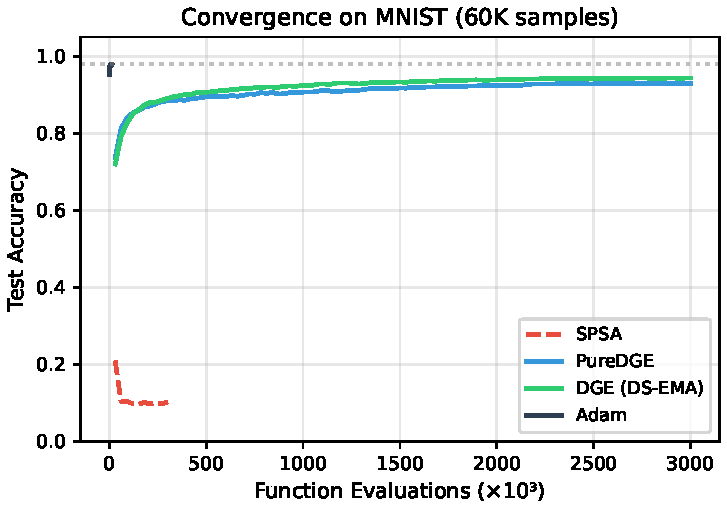
\includegraphics[width=0.72\linewidth]{convergence_mnist.pdf}
    \caption{\textbf{Convergence Trajectories on Full MNIST.} Test accuracy as a function of function evaluations. Global baselines (SPSA, MeZO) collapse due to excessive variance in 109K dimensions. DGE cleanly separates within 30K evaluations and reaches 94.36\% accuracy.}
    \label{fig:convergence}
\end{figure}

Global zeroth-order baselines collapse to near-chance performance (13.8\% for MeZO, 20.87\% for SPSA), corroborating the variance catastrophe. In sharp contrast, coordinate block partitioning alone elevates accuracy to 88.86\% (+75.06pp over MeZO), Adam second-moment scaling brings it to 93.00\%, and the DS-EMA consistency mask delivers the final refinement to \textbf{94.36\%~$\pm$~0.23\%} (Figure~\ref{fig:convergence}).

\subsection{Non-Differentiable and Quantized Neural Networks}
\label{sec:nondiff_results}

The primary technological advantage of DGE is its ability to optimize architectures that possess zero analytical gradients almost everywhere. We test three non-differentiable settings without using Straight-Through Estimators (STE):
\begin{enumerate}
    \item \textbf{Sign Activation Networks:} Replacing smooth activations with $h = \text{sign}(W x + b)$, creating flat step functions with zero derivative everywhere.
    \item \textbf{INT8 Full Quantization:} Symmetrically quantizing both weights and activations to 256 discrete levels ($[-127, +127]$).
    \item \textbf{INT4 Full Quantization:} Quantizing weights and activations to 16 discrete levels ($[-7, +7]$).
\end{enumerate}

\begin{table}[t]
\centering
\caption{\textbf{Non-Differentiable and Quantized Architectures (No STE).} Adam fails completely when analytical gradients are zero. DGE optimizes deep discrete representations natively.}
\label{tab:nondiff}
\resizebox{\linewidth}{!}{
\begin{tabular}{@{}lccc@{}}
\toprule
\textbf{Architecture / Precision} & \textbf{Adam (Backprop without STE)} & \textbf{DGE (Zeroth-Order)} & \textbf{Evaluation Budget} \\
\midrule
Sign activations ($\text{sign}(x)$) & 65.30\% & \textbf{70.43\%} & 200,000 \\
INT8 full quantization (256 levels) & 9.78\% (collapse) & \textbf{74.24\%} & 600,352 \\
INT4 full quantization (16 levels) & 9.82\% (collapse) & \textbf{68.82\%} & 600,352 \\
\bottomrule
\end{tabular}
}
\end{table}

\begin{figure}[t]
    \centering
    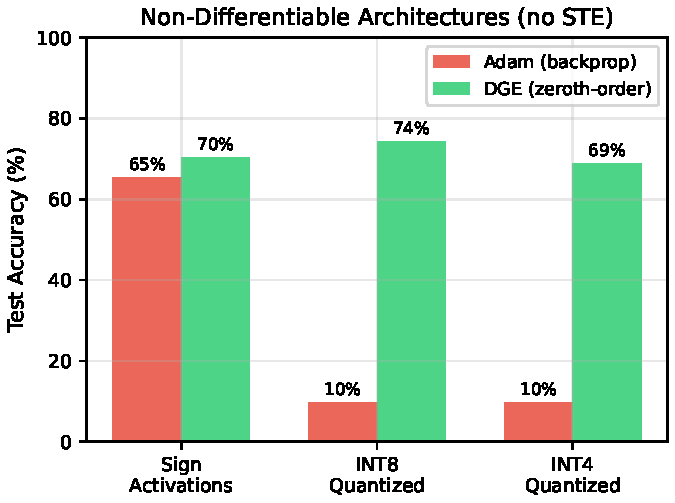
\includegraphics[width=0.68\linewidth]{non_diff_barplot.pdf}
    \caption{\textbf{Performance on Non-Differentiable Architectures.} Accuracy comparison between analytical backpropagation (Adam) and DGE without surrogate gradient heuristics.}
    \label{fig:nondiff}
\end{figure}

As shown in Table~\ref{tab:nondiff} and Figure~\ref{fig:nondiff}, backpropagation fails completely in INT8 and INT4 quantized networks ($\sim$9.8\% accuracy, equivalent to random classification), because the piecewise-constant floor functions produce zero gradients everywhere. DGE natively ascends the discrete loss landscape, achieving \textbf{74.24\%} on INT8 and \textbf{68.82\%} on INT4. On sign activations, Adam can only train the final linear layer (65.30\%), whereas DGE optimizes through all hidden layers to attain \textbf{70.43\%}.

\subsection{Rigorous Component Ablation Study}
\label{sec:ablation_results}

Figure~\ref{fig:ablation} isolates the incremental contribution of each component within the DGE optimization pipeline under identical test conditions.

\begin{figure}[t]
    \centering
    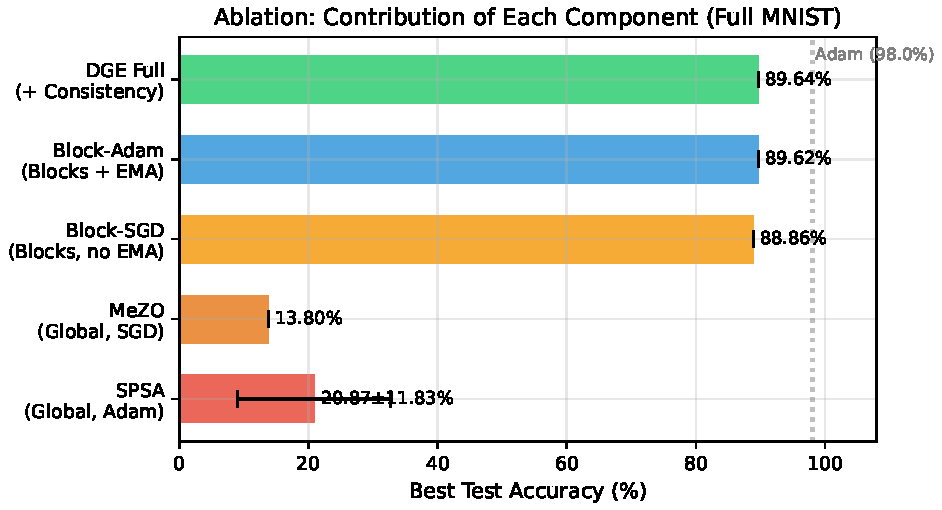
\includegraphics[width=0.75\linewidth]{ablation_components.pdf}
    \caption{\textbf{Component Ablation on Full MNIST.} Monotonic progression demonstrating the contribution of coordinate partitioning, adaptive momentum, and DS-EMA temporal filtering.}
    \label{fig:ablation}
\end{figure}

The empirical progression confirms the multi-stage theoretical architecture:
\begin{itemize}
    \item \textbf{MeZO (13.80\%) $\to$ SPSA (20.87\%):} Standard global zero-order updates diverge in 109K dimensions.
    \item \textbf{SPSA (20.87\%) $\to$ Block-SGD (88.86\%):} Coordinate blocking provides a massive \textbf{+67.99pp gain}, validating the $K$-fold variance reduction lemma.
    \item \textbf{Block-SGD (88.86\%) $\to$ Block-Adam (93.00\%):} Normalizing noisy zero-order gradients by coordinate-wise second moments adds \textbf{+4.14pp}.
    \item \textbf{Block-Adam (93.00\%) $\to$ DGE Full (94.36\%):} DS-EMA consistency gating filters out spurious gradient noise, providing the final \textbf{+1.36pp improvement}.
\end{itemize}

\subsection{Synthetic Benchmark Manifolds}
\label{sec:synthetic_results}

We validate the noise-rejection capability of DS-EMA across four ill-conditioned synthetic optimization landscapes ($D=128$, 200K evaluations, 5 random seeds), summarized in Table~\ref{tab:synthetic}.

\begin{table}[t]
\centering
\caption{\textbf{Final Loss on Synthetic Benchmarks (5 seeds, lower is better).} DS-EMA achieves superior or competitive convergence across diverse landscape curvatures.}
\label{tab:synthetic}
\resizebox{\linewidth}{!}{
\begin{tabular}{@{}lccc@{}}
\toprule
\textbf{Objective Function} & \textbf{PureDGE (No Mask)} & \textbf{Sliding Window ($T=20$)} & \textbf{DS-EMA (Ours)} \\
\midrule
Rosenbrock ($D=128$) & $1.40 \times 10^2$ & $1.14 \times 10^2$ & $\mathbf{1.06 \times 10^2}$ \\
Rotated Quadratic ($D=128$) & $2.82 \times 10^{-12}$ & $3.48 \times 10^{-9}$ & $\mathbf{1.49 \times 10^{-12}}$ \\
Ellipsoid ($\kappa = 10^6$) & $7.51 \times 10^3$ & $7.43 \times 10^2$ & $\mathbf{2.99 \times 10^2}$ \\
High-Dimensional Sphere ($D=8192$) & $6.81 \times 10^{-39}$ & $5.85 \times 10^{-29}$ & $\mathbf{2.43 \times 10^{-39}}$ \\
\bottomrule
\end{tabular}
}
\end{table}

On the Rotated Quadratic, sliding-window SMA degrades by three orders of magnitude ($3.48 \times 10^{-9}$) due to truncation boundary shocks when directional signs exit the window buffer. DS-EMA's continuous exponential smoothing eliminates these boundary effects, attaining $1.49 \times 10^{-12}$.

\begin{figure}[t]
    \centering
    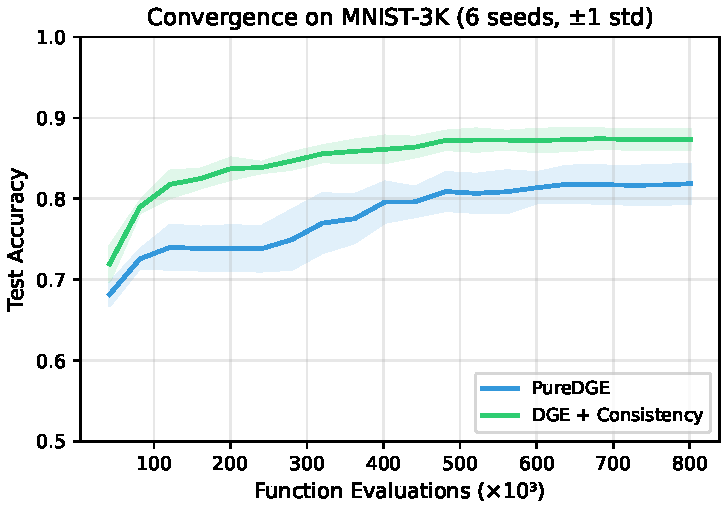
\includegraphics[width=0.72\linewidth]{convergence_6seeds.pdf}
    \caption{\textbf{Convergence on MNIST-3K Across 6 Seeds (Mean $\pm$ 1 Std).} DGE with consistency achieves 87.58\%~$\pm$~1.23\% vs.\ 82.22\%~$\pm$~2.25\% for PureDGE, reducing seed variance by 45\%.}
    \label{fig:convergence6}
\end{figure}

% -----------------------------------------------------------------------------
\section{Discussion: Systems, Memory, and Limitations}
\label{sec:discussion}
% -----------------------------------------------------------------------------

\paragraph{Computational and Wall-Clock Trade-offs.}
In fully differentiable settings where analytical derivatives are available, backpropagation remains superior in wall-clock convergence: Adam completes 30 training epochs in $\sim$19 seconds on our hardware, whereas DGE requires $\sim$13.5 minutes for 3,000,000 forward evaluations. However, when compared to traditional zeroth-order optimizers, DGE evaluates $10\times$ more perturbations than single-direction SPSA or MeZO while finishing in less than one-third of the wall-clock time ($\sim$13.5 min vs.\ $\sim$48 min for 300K SPSA steps). This runtime advantage stems directly from batching all $2K$ coordinate perturbations into vectorized tensor operations, amortizing GPU memory bandwidth and eliminating serial execution bottlenecks.

\paragraph{Memory Footprint Advantages.}
Standard backpropagation requires caching all intermediate layer activations during the forward pass in order to evaluate chain-rule Jacobian products during the backward pass. This activation cache scales linearly with network depth and batch size ($\mathcal{O}(L \cdot B)$), constituting over 70\% of peak VRAM during training. In contrast, DGE performs strictly forward inference passes; it requires zero activation caching, restricting memory complexity strictly to $\mathcal{O}(\text{parameters} + \text{batch})$. This makes DGE exceptionally well-suited for edge devices and microcontrollers with restricted on-chip SRAM.

\paragraph{Limitations and Failure Modes.}
We identify two primary limitations:
\begin{enumerate}
    \item \textbf{Deep Discrete Butterfly Effect:} In very deep discrete networks ($\ge 8$ layers), a perturbation in the initial layer can alter the binary state of all downstream features, disrupting the temporal landscape stationarity required by the EMA filter.
    \item \textbf{Conditioning in Discrete Landscapes:} While DGE trains INT4/INT8 networks effectively, performance remains below continuous 32-bit floating-point models ($\sim$74\% vs.\ 94\%). Developing curvature-aware adaptive block partitions represents a promising avenue to close this gap.
\end{enumerate}

% -----------------------------------------------------------------------------
\section{Conclusion}
\label{sec:conclusion}
% -----------------------------------------------------------------------------

We presented \textbf{Denoised Gradient Estimation} (DGE), a zeroth-order optimization algorithm capable of training deep neural networks without analytical backpropagation. By uniting coordinate block perturbations, temporal momentum filtering, and Dual Sign-EMA consistency gating, DGE overcomes the variance curse that has historically paralyzed zeroth-order methods in high-dimensional spaces.

DGE achieves 94.36\% accuracy on MNIST without gradients, and delivers robust performance on quantized (INT8/INT4) and sign-activation architectures where backpropagation fails completely without straight-through approximations. Requiring neither automatic differentiation nor activation memory caching, DGE establishes a rigorous, scalable foundation for optimization on neuromorphic processors, discrete computational fabrics, and black-box physical systems.

% -----------------------------------------------------------------------------
\bibliographystyle{plainnat}
\bibliography{references}
% -----------------------------------------------------------------------------

\end{document}
